\chapter{Implementation}
\label{cha:implementation}
\epigraph{
  \hypersetup{linkcolor=bgwhite}

This chapter describes the implementation and gives an overview of the translation of the FNN model to SME. The purpose is to show the structure and thoughts throughout the development of the final SME model. We will highlight the most important technical considerations made during the implementation and how the system was set given the previous chapters' theoretical background. This will be illustrated through explanations and code snippets.
%\hl{When the model is built up in SME, the next step would be to test the model by using simulations in SME. This is done straightforward, given that SME can handle floating points during the simulations. However, it does not work when implementing the model on hardware offered that SME is still taking floating points, so we need to quantize the data. To make this, several approaches had to be done.}



 % Chapter~\ref{cha:anomaly_detection};  
  \hypersetup{linkcolor=linkblue}
}

\iffalse
\section{Thoughts behind the implementation (IS this necessary??)}%
\label{sub:the_journey}

\hl{During the process of working on this thesis, I was not sure how much of the programming and hardware part I was able to learn and implement. However, it was interesting to see how a physicist lacking programming experience, especially with no experience in hardware design, could understand and build a structure of hardware working with high-level code. Therefore, a lot of time and energy was put into the computational parts such as learning - C\texthash, object-orientated programming, machine learning, simulations through SME, understanding time circuits, and generalizing everything such that it can be used for different FNN models and implemented on to an FPGA. My journey to the final code has been a development of exploring different structures and setups of the code, which has been rewritten and updated multiple times.} \\
\fi 

\section{The architecture of SME\_ML}%
\label{sec:SME_ML}
Having the theoretical background behind FNN and SME, we will in this section introduce the implementation of the FNN model in SME and describe some of the essential parts.
The code that was developed in this work \textbf{ML\_SME\_FPGA} can be found on Github [\cite{Github}]. The result is generalized such that each function can be used for different purposes on an FPGA.  
The ultimate goal is to find methods for transpiling that
can be generalized to different FNN problems.
The python code provided by the HFT company who wants to remain anonymous was made in python with the \emph{Pytorch} library, which I after that translated to C\#, using almost no built-in libraries. This was because we wanted to understand the data structure of all operations such that it would be easier to implement with SME.
The main intention of each language is different, and therefore the transpiling of a process in the given Python code to an SME process might not be completely trivial. However, the automatic parallelization of the network is still helpful for users wanting to run the model on an FPGA.
\\

Before getting into the concrete implementation detailing the model, let us restate the purpose of the FNN model and how we want to go from a Python model to full implementation on an FPGA.
Based on an input sequence $\mathbf{x}$ and a set of trained weights $\mathbf{w_i}$, a model is made to predict a $\mathbf{y}$ in Pytorch, which we will recreate in SME. We will do this by being aware of timing and restricted clock cycles such that the calculations run correctly and independently of each other. The final model works in the following way:

\begin{enumerate}
    \item \textbf{Takes in} the input sequence $\mathbf{x}$ and the weights $\mathbf{w_i}$. 
    \item \textbf{Runs} the FNN model
    \item \textbf{Compares} the SME- with the Pytorch -output
\end{enumerate}
The whole architecture is divided into several sections, but to execute this, you need to load your data in the \texttt{Deflib/data} file and run the \texttt{FNN} folder. The \texttt{FNN} calls in all the other modules, which can be found in \textbf{ML\_SME\_FPGA}. In the following sections, we will describe some specific implementation details worth noting. \\

\newpage

\section{Matrix multiplication in SME}
Each module is designed as an individual simulation setup to be tested separately from the rest of the system. A further explanation about how to test the modules can be found in Section~\ref{sec:simulation}.
To give an idea of how each function is structured in the core of the FNN, we will look at a concrete example; the \ttt{Matmul} function. 
To understand the development of the process, we will go through the steps of going from the python to SME model. This consists of the following main steps:

\begin{itemize}
    \item Translation from python to C\#
    \item Write in the SME framework
    \item Re-structure functions to run independently
\end{itemize}

\subsection{FNN in C\#}
For this example, we will only focus on this specific line from the given FNN model shown again in listing ~\ref{lst:mm}. This function calculates the matrix multiplication in the first layer of the model.
As we can see in listing \ref{lst:mm}, before the matrix multiplication, there is a need for a reshaping and transposing of the function, but we will only focus on the matrix multiplication for now. 
I had to write the function out in C\#.
This is generally not necessary to do first, but beneficial since it is needed for the testing. Another reason and something to be aware of is that this is done because in SME in specific situations, calling C\# libraries will not translate directly to VHDL, which is the goal. This happens when using the \texttt{SimpleProcess}. The global hidden clock drives this process with the OnTrigger function that is triggered once in each clock cycle [\cite{LennartJones}].
The \texttt{Matmul} function is shown in Listing~\ref{lst:mm_func}. Translating all lines to the necessary functions such as reshape, transpose, sigmoid, etc. It was done and tested with several examples to ensure it worked for different cases. I manually tested all functions to start with. This was my way to incorporate learning C\# programming. \\

The next step was recreating the FNN model in C\#, so it looked close to the python script. 
A snippet of the model from C\# is shown Listing~\ref{lst:mm_cs}.
Specific data was generated and tested a reasonable amount of times on both models to ensure that they both gave the same output. %This part could probably have been avoided if I had sufficient knowledge about machine learning and programming, but it was done for me to understand each step of the process and the structure of the code. Also, this made the SME part a notch easier to write.

\begin{listing}
  \inputminted{python}{codesnippets/mm.py}
  \caption{Matrix multiplication in python using the \texttt{Pytorch} library among other operations }
  \label{lst:mm}
\end{listing}

\begin{listing}
  \inputminted{csharp}{codesnippets/mm_func.cs}
  \caption{Matrix multiplication written out in C\# }
  \label{lst:mm_func}
\end{listing}


\iffalse
\begin{figure}[]
 \begin{minipage}{0.5\textwidth}
  \centering
   \inputminted{python}{codesnippets/mm.py}
  \captionof{listing}{Sub caption}
 \end{minipage}
 \begin{minipage}{0.6\textwidth}
  \centering
    \inputminted{csharp}{codesnippets/mm.cs}
  \captionof{listing}{Another sub caption}
 \end{minipage}
 \captionof{listing}{SomeCaption}
  \label{lst:representation_examples}
\end{figure}
\fi


\begin{listing}
  \inputminted{csharp}{codesnippets/mm.cs}
  \caption{The C\# version of listing \ref{lst:mm_func}}
  \label{lst:mm_cs}
\end{listing}

\section{Write to SME}
%This was the most challenging part of the work since the mindset behind hardware architecture was very new for me. 
The Sigmoid function was made to get introduced to the SME framework, which is shown in \ref{appendix:Sme_guide}. There are many ways to build a function in SME, and this was also the case for the \texttt{Matmul} process. Several block diagrams were made. The final block diagram is shown in Figure~\ref{fig:mm_block_old} containing the methods and busses that were necessary for the function to take in data, calculate correctly in the correct order and give an output. Because matrix multiplication is a combination of multiplication and addition, where the operations are dependent on each other, we need other functions to hold on to data and forward them. This is where the different processes come in. \\
The following sections will explain the different processes from the pipeline used in the implementation.


\begin{figure}
  \centering
  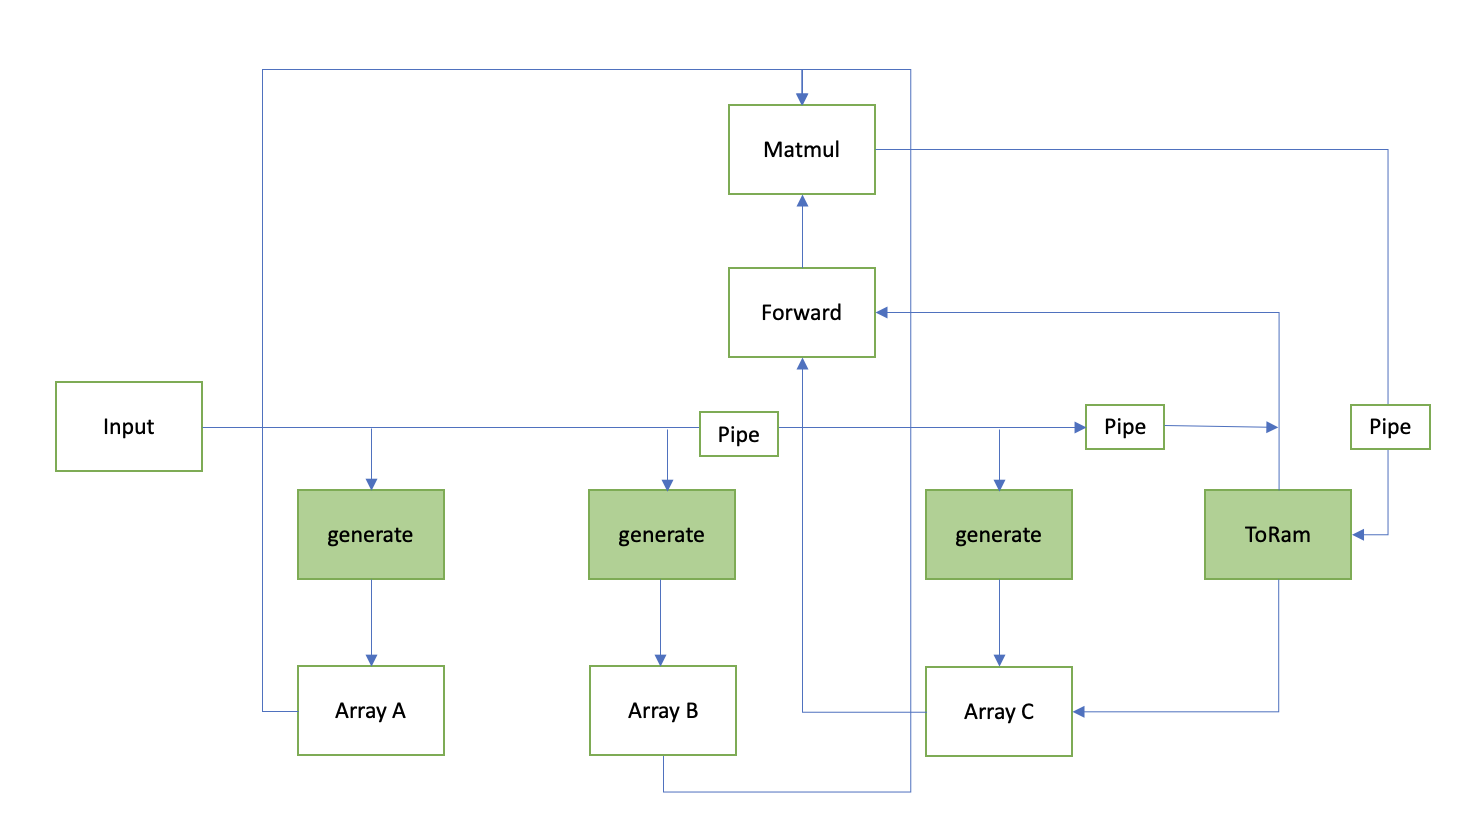
\includegraphics[width=1\linewidth]{Pictures/mm_block_old.png}
  \caption{Block diagram of the \texttt{Matmul} module. The colored boxes represent the non-clocked processes, since they just are empty 'boxes' with the only purpose of changing the bus type going through them.}
  \label{fig:mm_block_old}
\end{figure}

\subsection{Generate}
The generate function takes the data in their given sizes and outputs as a flat array since the $Ram$ only takes flat data. The actual shapes will be defined when addressing the data, i.e., in \texttt{MatmulIndex}. 
This process has an input bus that holds the base address, and the output bus reads the data.

\subsubsection{Implementation}
To implement the unit, we create an SME process. 
In SME, a process cannot make matrices from lists, as lists are dynamically allocated. However, we can make them as arrays as these can be statically allocated. It needs to be clocked, meaning the unit will activate on a rising clock edge, as it will be part of a closed-loop circuit when we later connect the units. If no unit is clocked in a closed-loop, there is no way of knowing where to begin sending signals, and if translated to hardware, one would get a short circuit, which would destroy the chip.
Because the process is clocked, when it reads the following address input, it will contain the address calculated in the previous clock cycle, as the bus has not been updated yet. This would then be the correct address in the current clock cycle.
This is because the bus has not been updated yet. This would then be the correct address in the current clock cycle. 

\begin{listing}
  \inputminted{csharp}{codesnippets/generate.cs}
  \caption{The generate process}
  \label{lst:datagenerator}
\end{listing}

\subsection{Matmul and Matmulindex}

\subsubsection{Matmul}
The \texttt{Matmul} is implemented as a pipeline, where each sub computation is performed in a single clock cycle.
The \texttt{Matmul} process takes in the Block RAM that holds the matrices, A and B used for the computation $C += A * B$. When C is calculated, it gets sent through the \texttt{Forward} process and will continue into the \texttt{Matmul}. When the calculation is ready, it will add C to the next A and B in the matrix. These ports are named Array\_A, Array\_B, and Array\_C, respectively, which are all input busses, meaning the data are stored in these arrays.

\subsubsection{Implementation}
This process takes four busses and outputs the calculated value.
Three input busses are the matrices Array\_A, Array\_B, and Array\_C.
It also consists of one input-bus, \emph{input\_pipe}, which is a base holding the base address. 
To give an idea of how a process looks like, we will show the whole \texttt{SimpleProcess} once, including how we define the busses and the structure of the process. The actual relevant part here is from line 28, where we define an \texttt{OnTick}. This is the part that runs over one clock cycle. If the following input is ready, we will calculate the matrix multiplication. With this, we can check if it takes data in. From now on, I will only show the \texttt{OnTick} functions since they are more relevant.
Additionally, since all data needs to be handled as flat lists for the matrices, we must define another process that keeps track of the real matrix shapes. This function is called \texttt{MatmulIndex}. 

\iffalse
\begin{listing}
  \inputminted{csharp}{codesnippets/Matmul_old.cs}
  \caption{The whole process for the \texttt{Matmul} calculations including the structure with busses used}
\end{listing}
\fi

\subsubsection{MatmulIndex}
\ttt{MatmulIndex} keeps track of the indices in the matrices. It can be thought of as a register that holds the current instruction's address. This is very important to keep track of where we are in the matrix. It is also here the dimensions of the matrices are being taken into account.
The input busses contains of \emph{controlA} and \emph{controlB}. The two control busses both contain a \texttt{bool} value which checks whether the dimensions of the input data are correct.
The output busses take the addresses from all the matrices, A, B, and C.
The last \emph{controlout} bus specifies the sizes and validity of the respective matrices.

\subsubsection{Implementation}

All the control busses are made from the \ttt{IndexControl} bus, which consists of the following fields: a boolean indicating whether the data is valid, a string holding the base address, an int indicating the access stride, and an int specifying the size of the matrix.
The main restriction with the \ttt{Matmul} function is the multiplication being dependent on the accumulation, which is performed within a single clock cycle. To make sure we hold the right data at the correct time, we add a process to the pipeline called \texttt{Forward}.


\begin{listing}
  \inputminted{csharp}{codesnippets/matmulind.cs}
  \caption{The Matmulindex }
  \label{lst:datagenerator}
\end{listing}



\iffalse
\begin{enumerate}
    \item \textbf{generate}
    \item \textbf{Matmulindex}, adressing the index in the matrices
    \item \textbf{pipe}
    \item \textbf{forward}
    \item \textbf{Matmul}
    \item \textbf{ToRam}
    
\end{enumerate}
\fi

\begin{figure}
    \centering
    \begin{tikzpicture}
        \node[block] (mem) at (0,0) {ToRam};
        \node[empty] (addr) at (-3,0.4) {Address};
        \node[empty] (data) at (-3,-0.4) {Data};

       
        \node[empty] (readdata) at (3, 0) {Read Data};

        \path[draw, ->] (addr) -- (mem.154);
        \path[draw, ->] (data) -- (mem.206);
        \path[draw, ->] (mem) -- (readdata);
    \end{tikzpicture}
    \caption{The ToRam Unit.}
    \label{fig:mem}
\end{figure}


\subsection{ToRam}
The ToRam Unit is like Generate, but for the write port to the memory. This is where the final calculations are stored. The FPGA can either read or write to the Memory
Unit in a single cycle. The Unit has two inputs: \ttt{v\_input} (the data) and \ttt{index} (the address).
It has a single output: \texttt{output}, where it writes the data. The ToRam Unit and its connections can be
seen in Figure~\ref{fig:mem}.

\subsubsection*{Implementation}
The ToRam process takes the Address and Data and should all contain a \texttt{int} value. 
The memory part should be an array, and
should read and write 
On each clock tick, the process should check if the \texttt{Index} flag is
set, in which case it should read the value on the Address bus and output the
the value stored in memory at the read address. 





 \subsection{Pipe}
Since parts of the Matmul function are dependent on its previous calculation,
there will be issues withholding the same positions in the indexing when running over each clock cycle. It is possible to write an indexing process in a way that reads and writes simultaneously; nevertheless, this will take a longer time when running the code. This is not very efficient, as the longest path in the processor determines the processor’s clock rate. A path
in a design is the components that a signal goes through until it reaches a
'ready' state. A ready state in an FPGA tells that the signals are safely
stored in the registers. A longer path implies a lower clock rate.
So to increase the clock rate, there is a need to decrease the longest path in the processor. For this, we introduce \ttt{Pipes}.\\
Pipes are registers in the processor, where all the values computed so far are
temporarily stored. It takes all of its inputs and holds them until the next
clock tick, where it will forward the values it is holding. This ensures that the data does not have to travel as far until it has reached a ready state.

\subsubsection*{Implementation}
Implementing the Pipe Unit should be done with an SME process. 
To implement the pipe function, we write the same function for the $genereate$ function.
On each clock tick, the process should check if the \texttt{Ready} flag is
set, in which case it should read the value on the Address bus and output the
the value stored in memory at the read address.


\subsection{Forwarding}
Since the Matmul calculation output depends on the previous output, we need to store the different outputs and require a process that can compare the other addresses and results and forward the final output.
The Forwarding Unit looks at the address $new\_input$ and check if the calculated value corresponds with the previous calculated address $old\_input$. If they fit, it will forward the calculated value 
from the \emph{Matmulindex} function to 
the Matmul stage. The structure of the simplified processor with the forwarding unit can be seen in Listing~\ref{lst:forward}.

\subsubsection*{Implementation}
Implementing the Forwarding Unit should be done with an SME process. As it
Interact with the Matmul stage should be put in the Matmul stage.
The unit consists of five busses.
The first four busses are input busses which we take in. They consist of two busses: the pipes that hold the $old\_input$ and $new\_input$ addresses. The following two busses are the calculated values of the old and new output, and the last bus is an output bus that forwards the value.


\begin{listing}
  \inputminted{csharp}{codesnippets/forward.cs}
  \caption{Forward process}
  \label{lst:forward}
\end{listing}


\section{The FNN model in SME}
For the rest of the needed functions in the network, the main challenge has been making sure that the right data and indices are correct.
However, they were built on the same principles, where the main difference in all of them was the structure of the processes sending the indices
around depending on size and dimension. 
The processes around the main functions in the FNN models, which are used more than once, are saved in the module \textbf{Deflib}. This is also where the data, simulation, and C\# version of the FNN models are kept. The rest of the relevant processes needed have their module.

When I first tested all the functions, they all depended on each other, leaving the debugging process very long and hard. Therefore there was a need to pipeline them all so that they could be modified and tested independently. 
All modules in the FNN simulation have been designed to be pipelined. This was an important design consideration because each module consisted of many individual calculations. If the system had to wait for each calculation to finish, it would increase the runtime considerably.
Each module setup consists of one or more \texttt{SimpleProcesses} and at least one \texttt{SimulationProcess} which generates input data for the network.
The pipelined structure results in each clock cycle, all sections of the modules are in use. The pipelined system also means that we cannot calculate something in one clock cycle and expect it still to be a couple of clock cycles down the line. This means that if a result from a calculation needs to be used later on, we either have to save it into the RAM or send it through the pipeline until it is required. With data always needed at a specific point in time, it makes sense to send it through the pipeline.
Understanding how a module can be built and connected leads us to the rest of the modules and their purpose in the FNN\_SME model. The raw connection between them is illustrated in fig.~\ref{fig:fnn_sme}. A lot of work was put into each module, making sure that it forwarded the correct data and sizes and ensuring that the calculations were executed at the correct time. The fully connected \acrshort{FNN} model can be seen in Figure~\ref{fig:fnn_block_sme}. The instructions on the addresses need to be given explicitly, such that everything gets sent around in the right order.
This means that no matter how much we try to generalize the modules, the addresses need to be changed if desired with the model. \\

Each module consists of a process, program, and simulation file. In the process file, there are two different processes. The first is the indexing of the input. Important notice when working with SME is that the dimensions are fixed to an extend. The biggest problem is that the RAM cannot change after the hardware has been generated. Processes such as index calculation are done dynamically and could easily be changed during run-time since they receive all of the dimensions on the control buses. If one were to truly fix all of the sizes, additional optimizations could be introduced since we don't have to have the complete precision given by a 32-bit number when there is only a need to count to 16.



\subsubsection{Transpose}
The transpose module is the only function not containing a natural process function since the function in itself changes the address of indices by transposing them.
To give a general idea of how the indexing process looks for most of the modules, an example of the \texttt{TransposeIndex} process is shown in Listing~\ref{lst:transpose}. The most relevant part in the indices getting addressed from lines 1-18. The rest are statements forwarding the information if the indexing holds. 

\begin{listing}
  \inputminted{csharp}{codesnippets/transpose.cs}
  \caption{Transpose index, addressing a }
  \label{lst:transpose}
\end{listing}



\begin{figure}
  \centering
  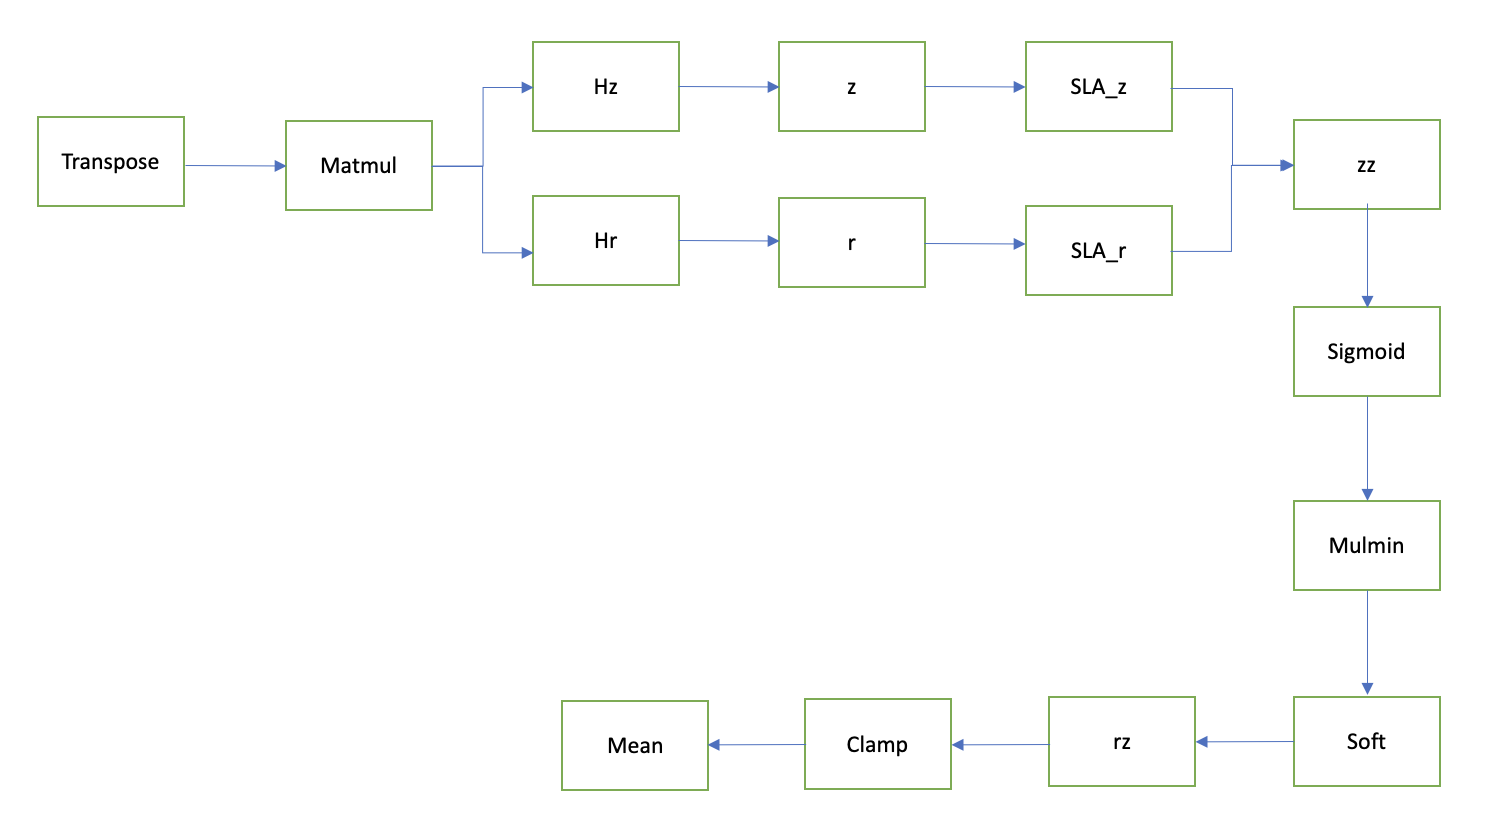
\includegraphics[width=1\linewidth]{Pictures/fnn_sme.png}
  \caption{
  }
  \label{fig:fnn_sme}
\end{figure}

\begin{figure}
  \centering
  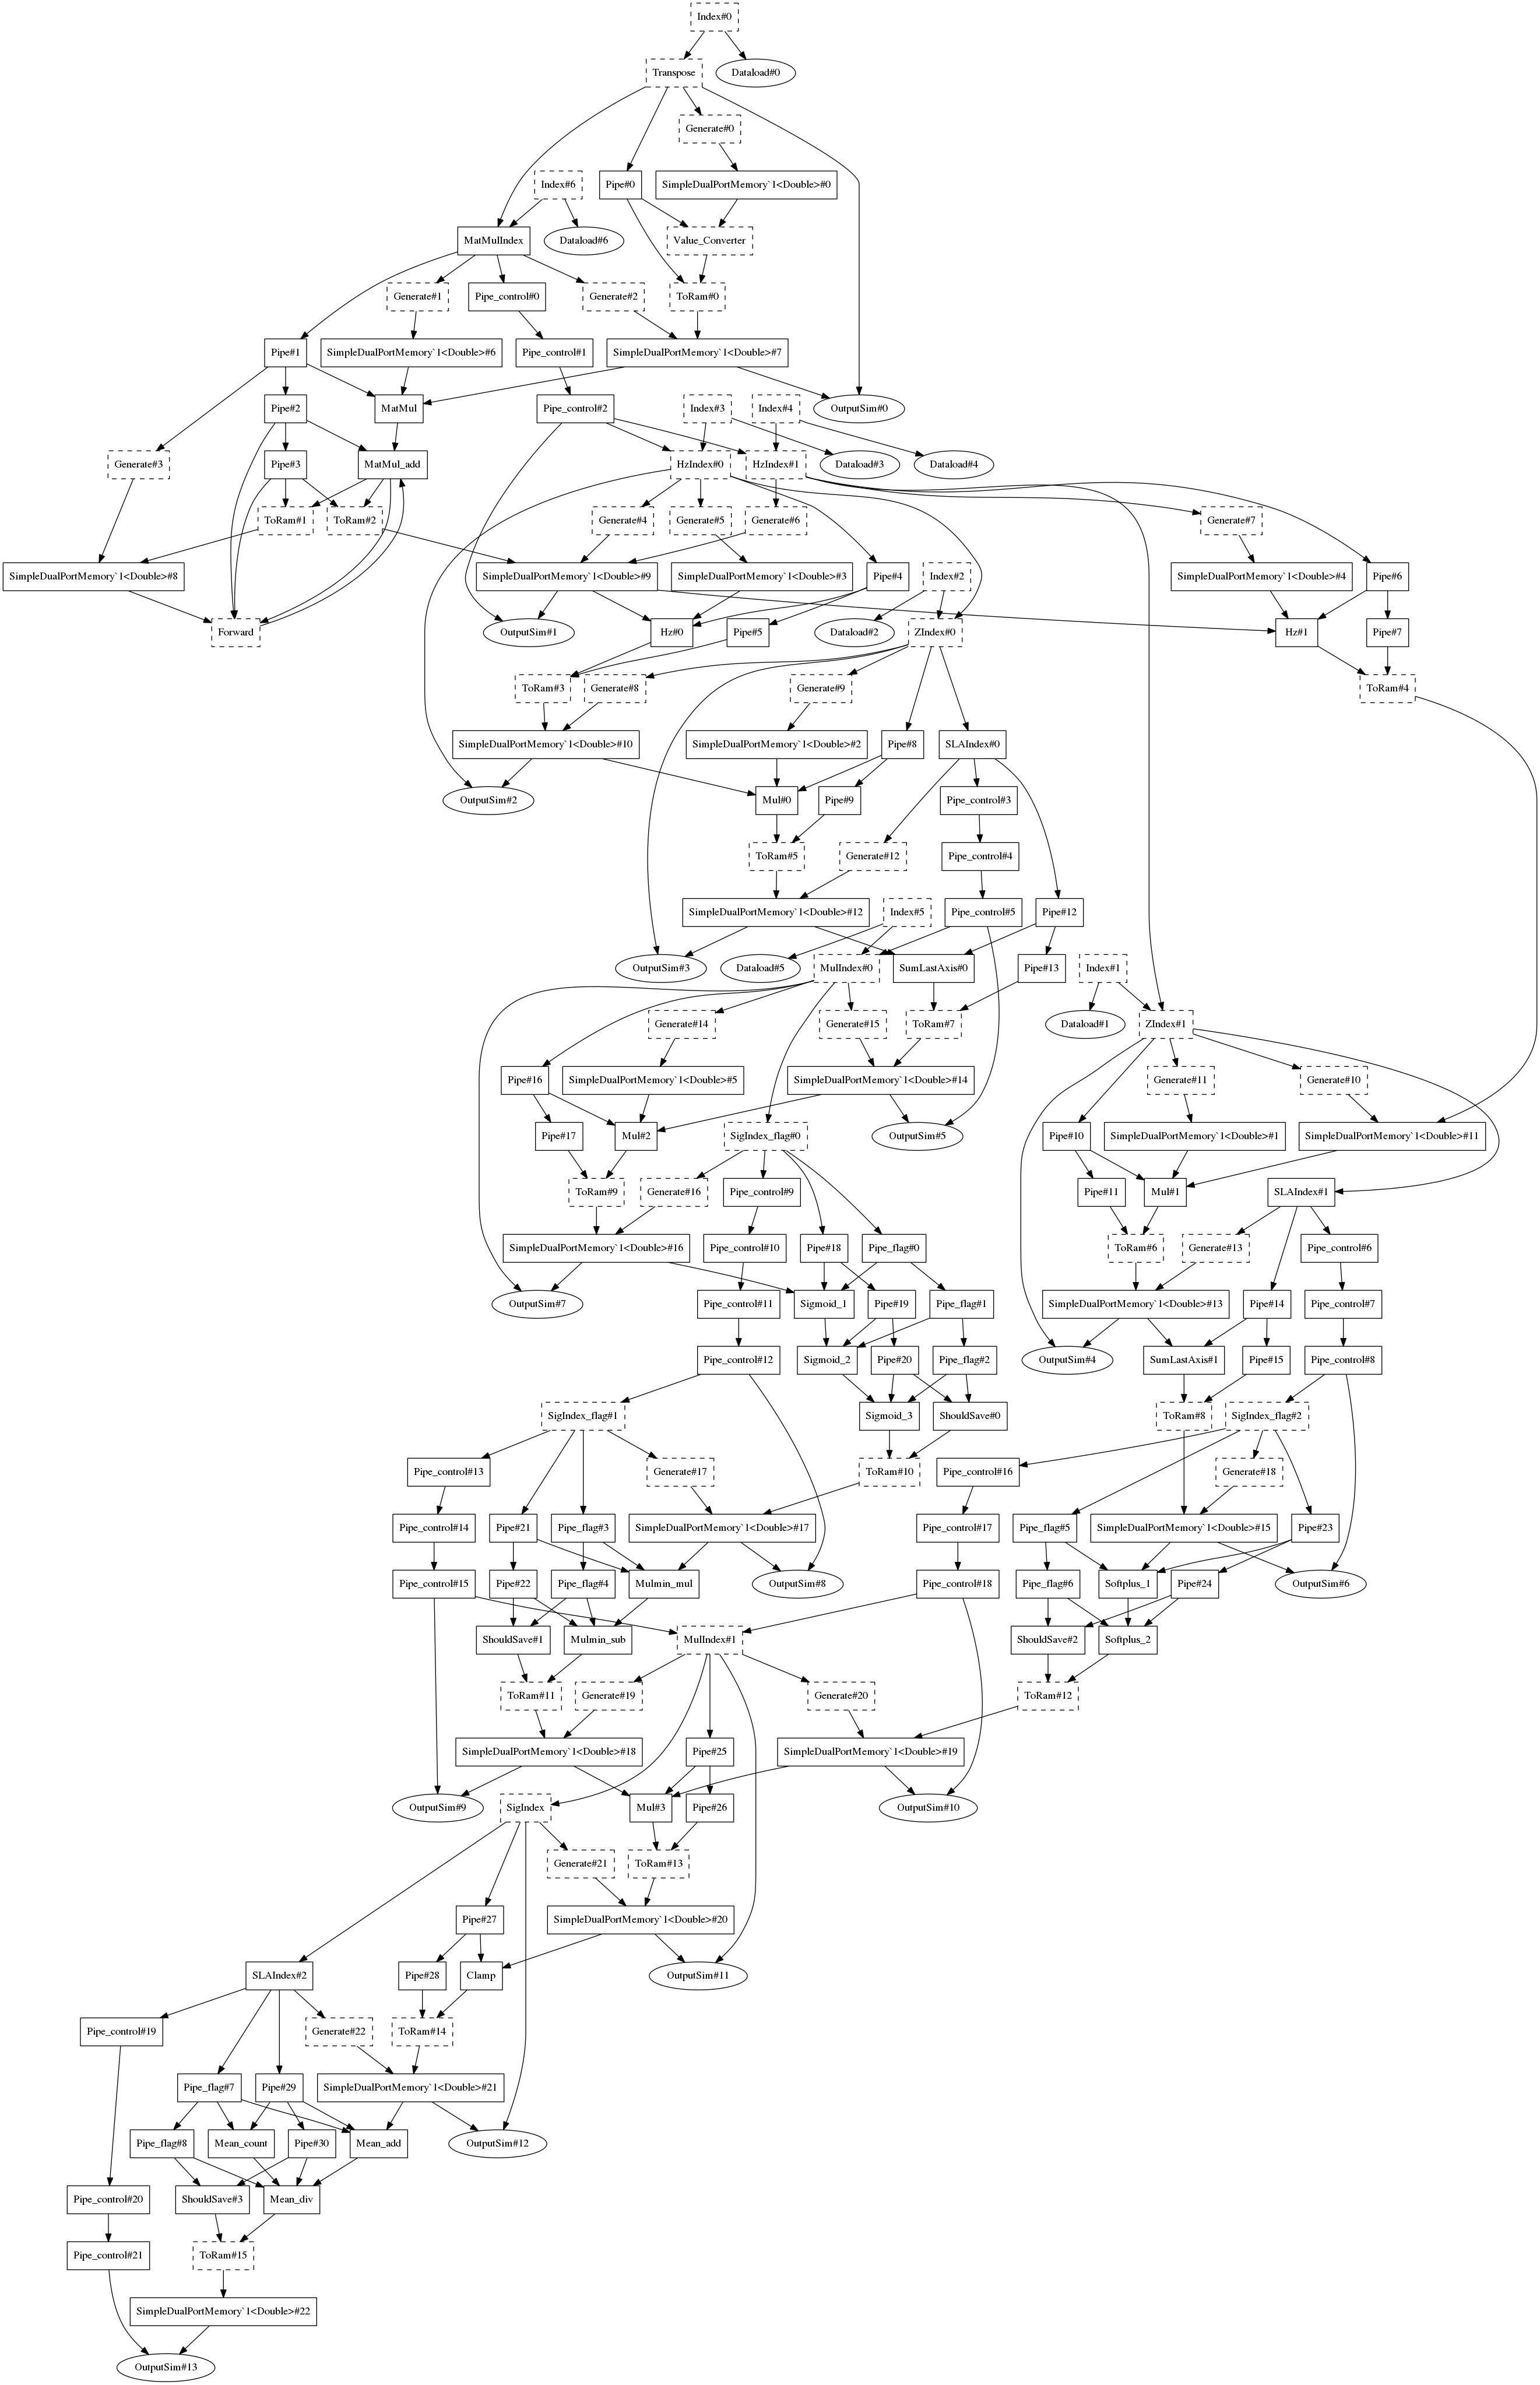
\includegraphics[width=1\linewidth]{Pictures/feedforward_diagram.png}
  \caption{Block diagram of the whole module  This diagram is not including all the busses used, but shows the connection of all the processes used}
  \label{fig:fnn_block_sme}
\end{figure}

\section{Quantization of Neural Networks}
\label{sub:quantization}
We are interested in comparing the results from the Pytorch model with the SME model, making sure that the functions are written correctly. However, the given data from the company is using floating points for their data. At the same time, the SME framework supports floats when simulating but does not yet have floating points implemented for deploying on an FPGA. One solution to compare the Pytorch and SME models would be to quantize the data in Python. \emph{Pytorch} has made it possible to quantize data while training the model. Quantization is a technique that stores tensors at lower bit widths than floating-point precision. A quantized model performs some or all of the operations on tensors with integers rather than floating-point values. This allows for a more compact model representation and the use of high-performance vectorized operations on many hardware platforms [\cite{quantization_pytorch}]. Quantization is primarily a technique to speed up inference, and only the forward pass is supported for quantized operators.
So to evaluate the data, we would need to train the models for quantization. Our focus is not really about training the model most efficiently but instead using it as a tool to get integers out.
The \emph{Pytorch} library arguments that it supports integer 8bit (INT8) quantization compared to typical floating-point 32bit models allowing for a 4x reduction in the model size and a 4x reduction in memory bandwidth requirements [\cite{quantization_pytorch}]. There are different approaches to quantizing the model depending on the whole pipeline structure: post-training dynamic quantization, post-training static quantization, and aware quantization training. Since this is just a tiny part of a more prominent structure, the simplest version would be enough to see if it works. \\

I chose to play with the python model to start with since this library seemed straightforward, but I must have missed something while working with it.
The instructions stated that applying the quantization on the model and training them would be needed to get a set of weighted integers. However, after several tries, the model wouldn't seem to save it any differently. I used the time to train the model and used all the different quantization approaches without any luck. Since this took too long to figure out and time was getting short, I decided to look into another way of getting the SME model to work with floating points. 


\section{ONNX}

An interesting thought that came up during this implementation was the question about saving \emph{Pytorch} models and uploading them directly in C\#, without translating manually and thereby saving a lot of time. 
With the PyTorch framework, it is possible to train a model, save it and download it as an ONNX file to run locally with Windows machine learning in C\#. This would save time for future work going from one framework to another and rewrite the C\# code into SME. 
We could also test other models containing the same operations we have implemented in SME and compare how fast they execute compared to each other.
This is where ONNX comes in handy. ONNX is an open format built to represent machine learning models. ONNX defines a standard set of the building blocks of machine learning and deep learning models. It generates a common file format to enable machine learning developers to use models with various frameworks, tools, run-times, and compilers.
We managed to save and download the model but could not open a translated \texttt{Pytorch} version in C\#. However, several attempts to use ONNX to convert different deep learning models were made without success. 

\newpage


\section{SME and floating points}
Since the time was running out, I decided to save this idea of optimizing the performance and focus on getting this piece of code working. 
Unlike with CPUs/GPUs, FPGAs are more limited in the available calculation methods, i.e., the SimpleProcess [\cite{LennartJones}]. We can not just import a math library to do advanced functions. Specific calculations have a drastically better performance than, e.g., division, and choosing wrong will reduce the performance of the system [\cite{LennartJones}]. Since we are targeting Xilinx boards, we are restricted to the \ac{IP} blocks that they provide for floating-point numbers. To be able to do calculations consisting of more than one operation in the \texttt{SimpleProcess} for the different modules used in the FNN model, we had to do some restructuring to fit it into the possible IP blocks provided by Xilinx. This means we will have to split the processes up into doing only one calculation, then several calculations in one process.\\

As an example, we will look at the \texttt{Matmul} function again. The original version of this process which calculates the \texttt{Matmul} consists of different operations such as accumulation and multiplications happening at the same time in the same process. However, if this should work for floating points, we will need to split it up so that the FPGA can more easily connect all operations.
This is therefor done by splitting the \texttt{Matmul} Process in two processes; \texttt{Matmul\_Add} and \texttt{Matmul\_Mul}.
On each clock cycle, one value is read from the A and B matrix, streamed to the Multiplier. The Accumulator keeps adding its input until the address for matrix C changes, writing the value to C. 
To ensure that all data gets sent at the proper clock cycle, some flags are set every time a result needs to be saved. We also need more pipes to hold the data until it is sent to the following process. The new structure of the matrix multiplication is shown as a block diagram in fig~\ref{fig:mm_diagram}. 


%På FPGA er floating-point enhederne lidt særlige, så for at det bliver effektivt skal værktøjet kunne gætte hvilke operationer der passer til hvilken hardware komponent. Ved at dele dem op til separate processer bliver det muligt for værktøjet at mappe dem korrekt.


\begin{figure}
  \centering
  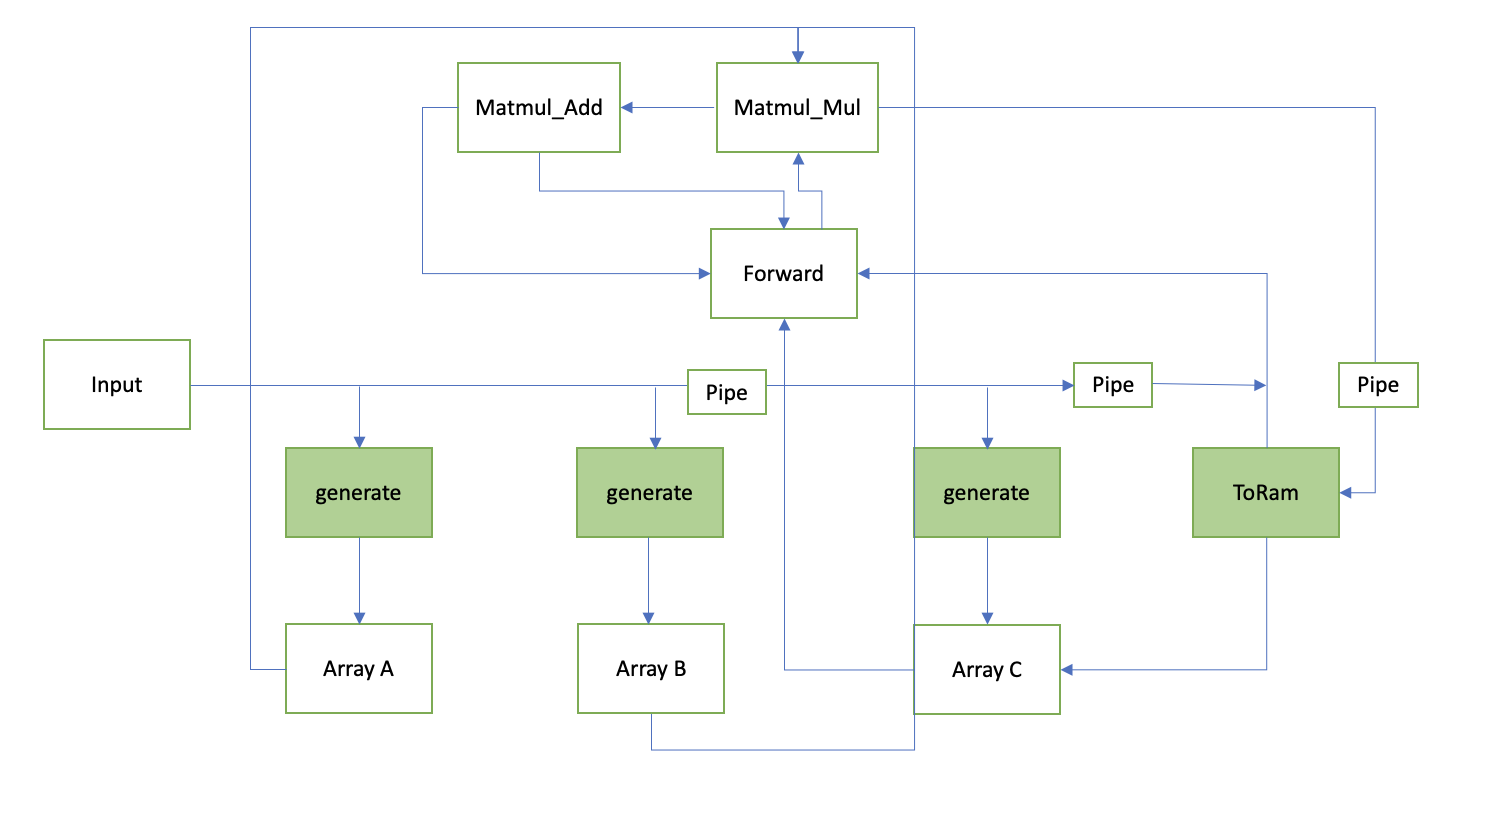
\includegraphics[width=0.8\linewidth]{Pictures/mm_blocks.png}
  \caption{Block diagram of the restructured \texttt{Matmul} module. The \texttt{Matmul} process is splitted up to \texttt{Matmul\_Add} and \texttt{Matmul\_Mul}}
  \label{fig:mm_diagram}
\end{figure}

\iffalse
\begin{listing}
  \inputminted{csharp}{codesnippets/mean_before.cs}
  \caption{Code snippet from the process calculating the mean before splitting up}
  \label{lst:mean_before}
\end{listing}


\begin{listing}
  \inputminted{csharp}{codesnippets/mean_after.cs}
  \caption{Codesnippet from the mean process calculation the mean}
  \label{lst:mean_after}
\end{listing}
\fi


\section{Simulation process}
\label{sec:simulation}

Now, having the structure of the SME feed-forward neural network model, we need to test whether or not it gives the same results as the \texttt{Pytorch} model.
There is a simulation part for each process to test the functions and follow the results. Notably, the final structure results from an iterative process, where the form of testing changed multiple times while building it.
The first simulation to test the functions was built to encompass all the other processes because nothing was pipe-lined and would therefore cause frequent errors. However, we managed to pipeline the structure, such that each module is designed as an individual simulation setup so that it can be tested separately from the whole system. When the modules are connected to the entire FNN network system, one \texttt{SimulationProcess} generates data and verifies the result.
Besides generating input data, the \texttt{SimulationProcess} uses self-made C\# libraries to calculate the results of the simulation as verification for the SME results. \\

Each module is a folder containing a \textbf{process.cs}, \textbf{program.cs} and \textbf{simulation.cs} file. The simulations file generates the expected output, and the test verification happens in \textbf{program.cs}. For instance, when calculating the \texttt{Sigmoid} function, the Testing Simulator will create input data generated from the calculation before, which is from the \texttt{zz} then. While the \texttt{Sigmoid} is calculated, the Testing Simulator will calculate the actual sigmoid function using standard C\#. This way, when \texttt{Sigmoid} gets computed, it is simple to check whether or not these results are as expected. The output will be a bool of true or false depending on if the results match. Often during development, we ran into errors where the calculations were correct, but the timing was wrong, which meant that the signals arrived unaligned, causing the results to be out of sync. By having a standard C\# calculation based on the current input data, it was easy to see how the timing of data communication was misaligned.

The Simulation is constructed using the following steps: A process that takes in the data converts the size and dimensions since the Ram only takes flattened data and simulates each function and compares it to the actual answer from the model.
With this in place, we can test each function and connect them. We are ultimately building the final FNN and testing it concurrently.

\subsection{LoadStage}
The \ttt{LoadStage} is a function that loads the data in, flattens it, and indexes it to the correct size and dimensions. It controls whether the index holds its proper size.
The \ttt{LoadStage} is shown in Listing~\ref{lst:loaddata} and consists of three other other processes:
\begin{itemize}
    \item DataLoad
    \item TestIndexSim
    \item Index
\end{itemize}

The \textbf{DataLoad }reads the CSV file, the total size of the data, and the value of the index. The output is a flat array ready to connect to a given address.
Since all the data comes in a flat array, we need to create a process that has the right dimensions to ensure that the sizes hold up. This is where \textbf{TestIndexSim} comes in. 
In \textbf{TestIndexSim} we overload with up to three dimensions including an index-control. The index control makes sure to output an error if the sizes do not hold up.
When we run the simulations, the sizes get transferred to the other processes with their given measures, which can then handle their actual dimensions.
The \textbf{index} keeps track of where in the program we are located. It can be thought of as a single register, which holds the address of the current instruction.
Further, the indexing process holds the instruction address. The input bus contains the address of the next instruction and the output bus with the current address.

\begin{listing}
  \inputminted{csharp}{codesnippets/loaddata.cs}
  \caption{LoadData process that loads the input and address the data with their correct sizes}
  \label{lst:loaddata}
\end{listing}

\subsection{simulation.cs}
When the data is loaded in with their correct sizes and dimensions, the next step would be to run them through the simulation processes.
Taking the structure of the \ttt{Matmul} Function as the starting point, there needs to be a simulation function to test out the results.
Before performing matrix multiplication, the model reshapes and transposes the data. The simulation process takes in the model, rewritten in C\#, and calculates the predicted outcome. In the \textbf{program.cs} file there are two parts:
The first part takes in all the SME processes written for that specific module and pipelines them to get the whole SME \ttt{Matmul} function; this part is called the \texttt{MatmulStage}. The other half of the \textbf{program.cs} takes in the data, the FNN network from both the C\# version and the SME and compares them inside the \ttt{OutputSim} process. 
The \textbf{OutputSim} is the process that compares the calculated output from SME with the expected output calculated using C\# functions.
To give a more straightforward visualization of the program file, a snippet of code is seen in Listing~\ref{lst:mm_program}.
Here, it calculates the expected Matmul output, generates the SME data, calculates the SME Matmul output, and compares those two at the end with \ttt{OutputSim.cs} which prints a \textbf{True} if the results match.\\


\begin{listing}
  \inputminted{csharp}{codesnippets/matmul_program.cs}
  \caption{Small snippet of code of the \texttt{program.cs} file calculating the matrix multiplication output for the expected and actual output}
  \label{lst:mm_program}
\end{listing} 




\label{sub:quantization}
%The given data from the company uses floating points on their data. The SME framework and does not yet have floating points Incorporated. This is why we need to quantize the data. \emph{Pytorch} has made it possible to do through the training of a model. Even though we evaluate the FNN model in SME, we will only train it in the python code for quantization. Our focus is not the training of the model but to quantizes the data and see if this also will help speed up the process of processing data. Since it is supposed to run faster for integers.\\
%Quantization refers to techniques for performing computations and storing tensors at lower bit widths than floating-point precision. A quantized model executes some or all of the operations on tensors with integers rather than floating-point values. This allows for a more compact model representation and the use of high-performance vectorized operations on many hardware platforms. PyTorch supports integer 8bit (INT8) quantization compared to typical floating-point 32bit (FP32)  models allowing for a 4x reduction in the model size and a 4x reduction in memory bandwidth requirements [\cite{quantization_pytorch}]. Quantization is primarily a technique to speed up inference, and only the forward pass is supported for quantized operators.
